\chapter{Appendix}
\label{anhang} 
\vspace{-7mm}
\begin{center}
\begin{minipage}{.8\textwidth}
	\begin{lstlisting}[numbers=left,
	stepnumber=1,caption={A Mutiple Nested Graph in GraphML},captionpos=b, linewidth={\textwidth}, escapeinside=||,label=GraphGraphML,gobble=4]
	<?xml version="1.0" encoding="UTF-8"?>
	<graphml xmlns="http://graphml.graphdrawing.org/xmlns">
	
		<graph id="G" edgedefault="undirected">
			<node id="n0"/>
			<node id="n1"/>
			<node id="n2"/>
			<node id="n6">
				<graph id="n6:" edgedefault="undirected">
					<node id="n6::n0">
					<graph id="n6::n0:" edgedefault="undirected">
						<node id="n6::n0::n0"/>
					</graph>
				</node>
					<node id="n6::n1"/>
					<node id="n6::n2"/>
					<edge id="e10" source="n6::n1" target="n6::n0::n0"/>
					<edge id="e11" source="n6::n1" target="n6::n2"/>
				</graph>
			</node>
			<edge id="e2" source="n5::n2" target="n0"/>
			<edge id="e3" source="n0" target="n2"/>
			<edge id="e8" source="n3" target="n6::n1"/>
			<edge id="e9" source="n6::n1" target="n4"/>
		</graph>
	</graphml>
	\end{lstlisting}
\end{minipage}
\end{center}

\begin{figure}
	\centering
	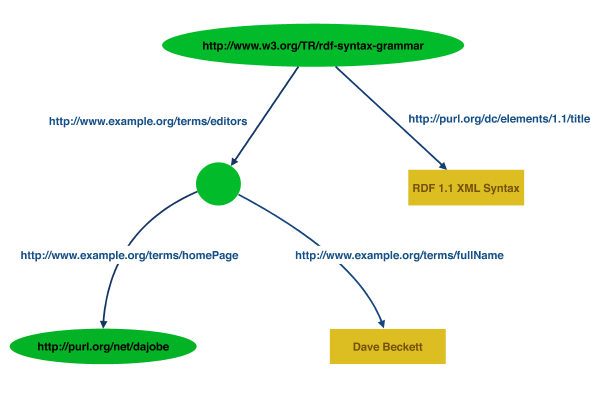
\includegraphics[width=1.0\linewidth]{img/rdf_graph.png}
	\caption{Graph in RDF}
	\label{GraphRDF}
\end{figure}
